\documentclass[lang=cn,10pt]{GorgeousnBook}

\title{Leonardo的ACM模板}
\subtitle{模板用的好,金牌少不了}

\author{列奥那多是勇者}
\institute{狗头吧}
\date{\today}
\version{$0.0.1$}
\bioinfo{邮箱}{azraelzarkli@gmail.com}

\extrainfo{狗头吧在什么时候都是acmer最好的救济}

\setcounter{tocdepth}{3}

\logo{avatar_bust.png}
\cover{cover.jpg}

% % 本文档命令
\usepackage{array}
\newcommand{\ccr}[1]{\makecell{{\color{#1}\rule{1cm}{1cm}}}}

% % 修改标题页的橙色带
\definecolor{customcolor}{RGB}{245, 250, 246}
\colorlet{coverlinecolor}{customcolor}
\usepackage{zhlipsum}
\usepackage{longtable}

\newif\ifshowLink % 是否显示题目链接的变量
\showLinktrue % 电子版最好设为true显示,打印版本应当设为false
% \showLinkfalse

\begin{document}


\chapterimage{catalog.png}
\maketitle
    \frontmatter
\thispagestyle{empty}
\newpage
\begin{center}
	\textbf{\LARGE 写在前面}
\end{center}
\begin{ascolorbox5}{模板使用须知}
本模板使用了 elegantbook-magic-revision latex模板( \href{https://github.com/Azure1210/elegantbook-magic-revision}{https://github.com/Azure1210/elegantbook-magic-revision}),在此对其表达感谢。\\
\ifshowLink
本文档的题显版本相关题目中包含AcWing题目,部分是需要买课才能查看的,这类题目可以到其它算法网站(如洛谷)上查找。
\fi

\end{ascolorbox5}

\frontmatter
\thispagestyle{fancy}
\tableofcontents

\mainmatter
\partsimage{part_0.png}
\part{STL}
\chapterimage{chapter_0.png}
\chapter{STL}

\begin{center}
    \pgfornament[width=0.36\linewidth,color=lsp]{88}
\end{center}

\begin{mybox1}
\textbf{备注}: 以c++14为标准
\end{mybox1}

\section{pair}
std::pair 是标准库中定义的一个类模板。用于将两个变量关联在一起,组成一个“对”,而且两个变量的数据类型可以是不同的。
\lstinputlisting[style=cpp]{code/stl/pair.cpp}

\section{vector}
std::vector 是 STL 提供的 内存连续的、可变长度 的数组(亦称列表)数据结构。能够提供线性复杂度的插入和删除,以及常数复杂度的随机访问。
\lstinputlisting[style=cpp]{code/stl/vector.cpp}

\section{array}
std::array 是 STL 提供的 内存连续的、固定长度 的数组数据结构。其本质是对原生数组的直接封装。
\lstinputlisting[style=cpp]{code/stl/array.cpp}

\section{deque}
std::deque 是 STL 提供的 双端队列 数据结构。能够提供线性复杂度的插入和删除,以及常数复杂度的随机访问。
\lstinputlisting[style=cpp]{code/stl/deque.cpp}

\section{list}
std::list 是 STL 提供的 双向链表 数据结构。能够提供线性复杂度的随机访问,以及常数复杂度的插入和删除。

list 的使用方法与 deque 基本相同,但是增删操作和访问的复杂度不同。此处列下特殊的(下列函数list提供了特别的实现以供使用):
\lstinputlisting[style=cpp]{code/stl/list.cpp}

\section{set / unordered\_set}
关于 unordered\_set 的哈希冲突,使用自定义哈希函数可以有效避免构造数据产生的大量哈希冲突,代码实现见本册附录。

set 是关联容器,含有键值类型对象的已排序集,搜索、移除和插入拥有对数复杂度。set 内部通常采用红黑树实现。平衡二叉树的特性使得 set 非常适合处理需要同时兼顾查找、插入与删除的情况。\\
和数学中的集合相似,set 中不会出现值相同的元素。如果需要有相同元素的集合,需要使用 multiset。multiset 的使用方法与 set 的使用方法基本相同。(当然也有unordered\_multiset)
\lstinputlisting[style=cpp]{code/stl/set.cpp}

\section{map / unordered\_map}
关于 unordered\_map 的哈希冲突,使用自定义哈希函数可以有效避免构造数据产生的大量哈希冲突,代码实现见本册附录。

map 是有序键值对容器,它的元素的键是唯一的。搜索、移除和插入操作拥有对数复杂度。map 通常实现为红黑树。multimap则允许有重复的Key值。(当然也有 unordered\_multimap)
\lstinputlisting[style=cpp]{code/stl/map.cpp}

\section{string}
std::string 是在标准库 <string>(注意不是 C 语言中的 <string.h> 库)中提供的一个类,本质上是 std::basic\_string<char> 的别称。

\lstinputlisting[style=cpp]{code/stl/string.cpp}

\section{stack}
STL 栈 (std::stack) 是一种后进先出 (Last In, First Out) 的容器适配器,仅支持查询或删除最后一个加入的元素(栈顶元素),不支持随机访问,且为了保证数据的严格有序性,不支持迭代器。
\lstinputlisting[style=cpp]{code/stl/stack.cpp}

\section{queue}
STL 队列 (std::queue) 是一种先进先出 (First In, First Out) 的容器适配器,仅支持查询或删除第一个加入的元素(队首元素),不支持随机访问,且为了保证数据的严格有序性,不支持迭代器。
\lstinputlisting[style=cpp]{code/stl/queue.cpp}

\section{priority\_queue}
默认容器为vector, 默认算子为 less, 也就是最大堆
\lstinputlisting[style=cpp]{code/stl/priority_queue.cpp}


\section{bitset}
std::bitset 是标准库中的一个存储 0/1 的大小不可变容器。严格来讲,它并不属于 STL。
\lstinputlisting[style=cpp]{code/stl/bitset.cpp}

\section{iterator}
\lstinputlisting[style=cpp]{code/stl/iterator.cpp}

\section{algorithm}

\subsection{Non-modifying sequence operations}

\begin{center}
\begin{longtable}{ll}
    \caption{Non-modifying sequence operations} \\
    \hline
        \textbf{operations} & \textbf{ functions } \\ \hline
        \hword{all\_of} \hword{any\_of} \hword{none\_of} & checks if a predicate is \textbf{true} for all, any or none of the elements in a range \\ \hline
        \hword{for\_each} & 	applies a function to a range of elements \\ \hline
        \hword{count} \hword{count\_if} & returns the number of elements satisfying specific criteria \\ \hline
        \hword{mismatch} & finds the first position where two ranges differ \\ \hline
        \hword{find} \hword{find\_if} \hword{find\_if\_not} & 	finds the first element satisfying specific criteria \\ \hline
        \hword{find\_end} &  finds the last sequence of elements in a certain range \\ \hline
        \hword{find\_first\_of} & searches for any one of a set of elements \\ \hline
        \hword{adjacent\_find} & finds the first two adjacent items that are equal (or satisfy a given predicate) \\ \hline
        \hword{search} & searches for a range of elements \\ \hline
        \hword{search\_n} & searches a range for a number of consecutive copies of an element \\ \hline
\end{longtable}
\end{center}

\lstinputlisting[style=cpp]{code/stl/algorithm/non-modifying.cpp}

\subsection{Modifying sequence operations}

\begin{center}
\begin{longtable}{ll}
    \caption{Modifying sequence operations} \\
    % \renewcommand\arraystretch{1.3}
    % \begin{tabular}{|l|l|}
    \hline
        \textbf{operations} & \textbf{ functions } \\ \hline
        \hword{copy} \hword{copy\_if} & copies a range of elements to a new location \\ \hline
        \hword{copy\_n} & copies a number of elements to a new location \\ \hline
        \hword{copy\_backward} & copies a range of elements in backwards order \\ \hline
        \hword{move} & moves a range of elements to a new location \\ \hline
        \hword{move\_backward} & moves a range of elements to a new location in backwards order \\ \hline
        \hword{fill} & copy-assigns the given value to every element in a range \\ \hline
        \hword{fill\_n} & copy-assigns the given value to N elements in a range \\ \hline
        \hword{transform} & assigns the results of successive function calls to every element in a range \\ \hline
        \hword{generate} & assigns the results of successive function calls to every element in a range \\ \hline
        \hword{generate\_n} & assigns the results of successive function calls to N elements in a range \\ \hline
        \hword{remove} \hword{remove\_if} & removes elements satisfying specific criteria \\ \hline
        \hword{remove\_copy} \hword{remove\_copy\_if} & copies a range of elements omitting those that satisfy specific criteria \\ \hline
        \hword{replace} \hword{replace\_if} & replaces all values satisfying specific criteria with another value \\ \hline
        \hword{replace\_copy} \hword{replace\_copy\_if} & copies a range, replacing elements satisfying specific criteria with another value \\ \hline
        \hword{swap} & swaps the values of two objects \\ \hline
        \hword{swap\_ranges} & swaps two ranges of elements \\ \hline
        \hword{iter\_swap} & swaps the elements pointed to by two iterators \\ \hline
        \hword{reverse} & reverses the order of elements in a range \\ \hline
        \hword{reverse\_copy} & creates a copy of a range that is reversed \\ \hline
        \hword{rotate} & rotates the order of elements in a range \\ \hline
        \hword{rotate\_copy} & copies and rotate a range of elements \\ \hline
        \hword{shuffle} & randomly re-orders elements in a range \\ \hline
        \hword{unique} & removes consecutive duplicate elements in a range \\ \hline
        \hword{unique\_copy} & creates a copy of some range of elements that contains no consecutive duplicates \\ \hline
    % \end{tabular}
\end{longtable}
\end{center}

\lstinputlisting[style=cpp]{code/stl/algorithm/modifying.cpp}

\subsection{Partitioning operations}

\begin{center}
\begin{longtable}{ll}
    \caption{Modifying sequence operations} \\
    \hline
        \textbf{operations} & \textbf{ functions } \\ \hline
        \hword{is\_partitioned} & determines if the range is partitioned by the given predicate \\ \hline
        \hword{partition} & divides a range of elements into two groups \\ \hline
        \hword{partition\_copy} & copies a range dividing the elements into two groups \\ \hline
        \hword{stable\_partition} & divides elements into two groups while preserving their relative order \\ \hline
        \hword{partition\_point} & locates the partition point of a partitioned range \\ \hline
\end{longtable}
\end{center}

\subsection{Sorting operations}

\begin{center}
\begin{longtable}{ll}
    \caption{Modifying sequence operations} \\
    \hline
        \textbf{operations} & \textbf{ functions } \\ \hline
        \hword{is\_sorted} & checks whether a range is sorted into ascending order \\ \hline
        \hword{is\_sorted\_until} & finds the largest sorted subrange \\ \hline
        \hword{sort} & sorts a range into ascending order \\ \hline
        \hword{partial\_sort} & sorts the first N elements of a range \\ \hline
        \hword{partial\_sort\_copy} & copies and partially sorts a range of elements \\ \hline
        \hword{stable\_sort} & sorts a range of elements while preserving order between equal elements \\ \hline
        \hword{nth\_element} & partially sorts the given range making sure that it is partitioned by the given element \\ \hline
\end{longtable}
\end{center}

\subsection{Binary search operations (on sorted ranges)}

\begin{center}
\begin{longtable}{ll}
    \caption{Modifying sequence operations} \\
    \hline
        \textbf{operations} & \textbf{ functions } \\ \hline
        \hword{lower\_bound} & returns an iterator to the first element not less than the given value \\ \hline
        \hword{upper\_bound} & returns an iterator to the first element greater than a certain value \\ \hline
        \hword{binary\_search} & determines if an element exists in a partially-ordered range \\ \hline
        \hword{equal\_range} & returns range of elements matching a specific key \\ \hline
\end{longtable}
\end{center}

\subsection{Other operations on sorted ranges}

\begin{center}
\begin{longtable}{ll}
    \caption{Modifying sequence operations} \\
    \hline
        \textbf{operations} & \textbf{ functions } \\ \hline
        \hword{merge} & merges two sorted ranges \\ \hline
        \hword{inplace\_merge} & merges two ordered ranges in-place \\ \hline
\end{longtable}
\end{center}

\subsection{Set operations (on sorted ranges)}

\begin{center}
\begin{longtable}{ll}
    \caption{Modifying sequence operations} \\
    \hline
        \textbf{operations} & \textbf{ functions } \\ \hline
        \hword{includes} & returns true if one sequence is a subsequence of another \\ \hline
        \hword{set\_difference} & computes the difference between two sets \\ \hline
        \hword{set\_intersection} & computes the intersection of two sets \\ \hline
        \hword{set\_symmetric\_difference} & computes the symmetric difference between two sets \\ \hline
        \hword{set\_union} & computes the union of two sets \\ \hline
\end{longtable}
\end{center}

\subsection{Heap operations}

\begin{center}
\begin{longtable}{ll}
    \caption{Modifying sequence operations} \\
    \hline
        \textbf{operations} & \textbf{ functions } \\ \hline
        \hword{is\_heap} & checks if the given range is a max heap \\ \hline
        \hword{is\_heap\_until} & finds the largest subrange that is a max heap \\ \hline
        \hword{make\_heap} & creates a max heap out of a range of elements \\ \hline
        \hword{push\_heap} & adds an element to a max heap \\ \hline
        \hword{pop\_heap} & removes the largest element from a max heap \\ \hline
        \hword{sort\_heap} & turns a max heap into a range of elements sorted in ascending order \\ \hline
\end{longtable}
\end{center}

\subsection{Minimum/maximum operations}

\begin{center}
\begin{longtable}{ll}
    \caption{Modifying sequence operations} \\
    \hline
        \textbf{operations} & \textbf{ functions } \\ \hline
        \hword{max} & returns the greater of the given values \\ \hline
        \hword{max\_element} & returns the largest element in a range \\ \hline
        \hword{min} & returns the smaller of the given values \\ \hline
        \hword{min\_element} & returns the smallest element in a range \\ \hline
        \hword{minmax} & returns the smaller and larger of two elements \\ \hline
        \hword{minmax\_element} & returns the smallest and the largest elements in a range \\ \hline
\end{longtable}
\end{center}

\subsection{Comparison operations}

\begin{center}
\begin{longtable}{ll}
    \caption{Modifying sequence operations} \\
    \hline
        \textbf{operations} & \textbf{ functions } \\ \hline
        \hword{equal} & determines if two sets of elements are the same \\ \hline
        \hword{lexicographical\_compare} & returns true if one range is lexicographically less than another \\ \hline
\end{longtable}
\end{center}

\subsection{Permutation operations}

\begin{center}
\begin{longtable}{ll}
    \caption{Modifying sequence operations} \\
    \hline
        \textbf{operations} & \textbf{ functions } \\ \hline
        \hword{is\_permutation} & determines if a sequence is a permutation of another sequence \\ \hline
        \hword{next\_permutation} & generates the next greater lexicographic permutation of a range of elements \\ \hline
        \hword{prev\_permutation} & generates the next smaller lexicographic permutation of a range of elements \\ \hline
\end{longtable}
\end{center}

\subsection{Numeric operations}

\begin{center}
\begin{longtable}{ll}
    \caption{Modifying sequence operations} \\
    \hline
        \textbf{operations} & \textbf{ functions } \\ \hline
        \hword{iota} & fills a range with successive increments of the starting value \\ \hline
        \hword{accumulate} & sums up a range of elements \\ \hline
        \hword{inner\_product} & computes the inner product of two ranges of elements \\ \hline
        \hword{adjacent\_difference} & computes the differences between adjacent elements in a range \\ \hline
        \hword{partial\_sum} & computes the partial sum of a range of elements \\ \hline
\end{longtable}
\end{center}

% \subsection{Operations on uninitialized memory}


% \section{numeric}
% cmath

\partsimage{part_6.png}
\part{数据结构}
\chapterimage{chapter_2.png}
\chapter{数据结构}

\begin{center}
    \pgfornament[width=0.36\linewidth,color=lsp]{88}
\end{center}

\section{并查集 DSU/UF}
\textbf{DSU}: Disjoint Set Union; \textbf{UF}: Union Find
并查集是一种树形的数据结构,顾名思义,它用于处理一些不交集的 合并 及 查询 问题。 它支持两种操作: 

\begin{itemize}
    \item 合并(Union):将两个子集合并成一个集合。
    \item 查找(Find):确定某个元素处于哪个子集;
\end{itemize}

\lstinputlisting[style=cpp]{code/data_structure/union_find.cpp}

\ifshowLink
讲解: \href{https://labuladong.github.io/algo/2/22/53/}{https://labuladong.github.io/algo/2/22/53/}\\
相关题目:
    \begin{enumerate}
        \item LeetCode 990. Satisfiability of Equality Equations: \href{https://leetcode.cn/problems/satisfiability-of-equality-equations/}{https://leetcode.cn/problems/satisfiability-of-equality-equations/}
    \end{enumerate}
\fi

\partsimage{part_1.png}
\part{基础算法}
\chapterimage{chapter_4.png}
\chapter{基础算法}

\begin{center}
    \pgfornament[width=0.36\linewidth,color=lsp]{88}
\end{center}

\section{排序算法}
\subsection{快速排序}
\lstinputlisting[style=cpp]{code/basic/sort/quick_sort.cpp}

\subsection{归并排序}
\lstinputlisting[style=cpp]{code/basic/sort/merge_sort.cpp}

\ifshowLink
相关题目:
    \begin{enumerate}
        \item AcWing 788. 逆序对的数量: \href{https://www.acwing.com/problem/content/790/}{https://www.acwing.com/problem/content/790/}
    \end{enumerate}
\fi

\section{二分}
\subsection{整数二分}
\lstinputlisting[style=cpp]{code/basic/binary_search/int.cpp}

\subsection{浮点数二分}
\lstinputlisting[style=cpp]{code/basic/binary_search/float.cpp}

\ifshowLink
相关题目:
    \begin{enumerate}
        \item AcWing 790. 数的三次方根: \href{https://www.acwing.com/activity/content/problem/content/824/}{https://www.acwing.com/activity/content/problem/content/824/}
    \end{enumerate}
\fi

\section{高精度}
也就是数比较大,不能放在通常的类型中的时候(像python, java 这类的语言本身就实现了这类性质)
\subsection{加法}
\lstinputlisting[style=cpp]{code/basic/high_eps/add.cpp}
\subsection{减法}
\lstinputlisting[style=cpp]{code/basic/high_eps/sub.cpp}
\subsection{乘法}
高精度乘低精度 如 10000位的乘以一个大小为100的
\lstinputlisting[style=cpp]{code/basic/high_eps/multiply.cpp}
\subsection{除法}
高精度除以低精度 如 10000位的除以一个大小为100的
\lstinputlisting[style=cpp]{code/basic/high_eps/div.cpp}

\section{前缀和}
\lstinputlisting[style=cpp]{code/basic/partial_sum.cpp}

\section{差分}
\lstinputlisting[style=cpp]{code/basic/difference.cpp}

\section{位运算}
oi-wiki: \href{https://oi-wiki.org/math/bit/}{https://oi-wiki.org/math/bit/}
\begin{enumerate}
    \item 异或运算的逆运算是它本身,也就是说两次异或同一个数最后结果不变,即 $a \ xor \  b \ xor \  b = 0$。
    \item 操作二进制的某位
    \lstinputlisting[style=cpp]{code/basic/bits/1.cpp}
    \item 判断两非零数符号是否相同
    \lstinputlisting[style=cpp]{code/basic/bits/2.cpp}
    \item 求n的第k位数字
    \lstinputlisting[style=cpp]{code/basic/bits/3.cpp}
    \item 返回n的最后一位1
    \lstinputlisting[style=cpp]{code/basic/bits/4.cpp}
    \item 模拟集合操作 \\
    一个数的二进制表示可以看作是一个集合(0表示不在集合中,1表示在集合中)。比如集合${1,3,4,8}$,可以表示成$(100011010)_{2}$。而对应的位运算也就可以看作是对集合进行的操作。更多见\textit{oi-wiki}
\end{enumerate}

\section{双指针算法}
\textbf{常见问题分类}:
\begin{enumerate}
    \item 对于一个序列,用两个指针维护一段区间 
    \item 对于两个序列,维护某种次序,比如归并排序中合并两个有序序列的操作  
\end{enumerate}
\lstinputlisting[style=cpp]{code/basic/double_pointer.cpp}

\section{离散化}
一般用于给定围很大,但所需范围较小的题
\lstinputlisting[style=cpp]{code/basic/discretization.cpp}

\ifshowLink
相关题目:
    \begin{enumerate}
        \item AcWing 802. 区间和: \href{https://www.acwing.com/problem/content/804/}{https://www.acwing.com/problem/content/804/}
    \end{enumerate}
\fi

\section{区间合并}
\lstinputlisting[style=cpp]{code/basic/interval_merge.cpp}


\partsimage{part_4.png}
\part{进阶算法}
\chapterimage{chapter_3.png}
\chapter{图论}
\begin{center}
    \pgfornament[width=0.36\linewidth,color=lsp]{88}
\end{center}

\section{二分图}
二分图常用来判断是否能分成两组

\subsection{检测二分图}
\lstinputlisting[style=cpp]{code/graph/isbipartition.cpp}

\ifshowLink
相关题目:
    \begin{enumerate}
        \item LeetCode 886. Possible Bipartition: \href{https://leetcode.cn/problems/possible-bipartition/}{https://leetcode.cn/problems/possible-bipartition/}
    \end{enumerate}
\fi
% \input{chapter/2_graph.tex} 进阶部分比较多,每章分开来



\partsimage{part_3.png}
\part{附录}
\chapterimage{chapter_5.png}
\chapter{附录}

\begin{center}
    \pgfornament[width=0.36\linewidth,color=lsp]{88}
\end{center}

\section{比赛初始代码模板}
\lstinputlisting[style=cpp]{code/competition.cpp}

\section{unordered\_set/map 哈希函数}
\lstinputlisting[style=cpp]{code/hash.cpp}
写完自定义的哈希函数后,就可以通过 unordered\_map<int, int, my\_hash> my\_map; 或者 unordered\_map<pair<int, int>, int, my\_hash> my\_pair\_map; 的定义方式将自定义的哈希函数传入容器了。

\section{Big-O Cheat Sheet}

\subsection{Common Data Structure Operations}
\begin{figure}[H] %H为当前位置,!htb为忽略美学标准,htbp为浮动图形
\centering %图片居中
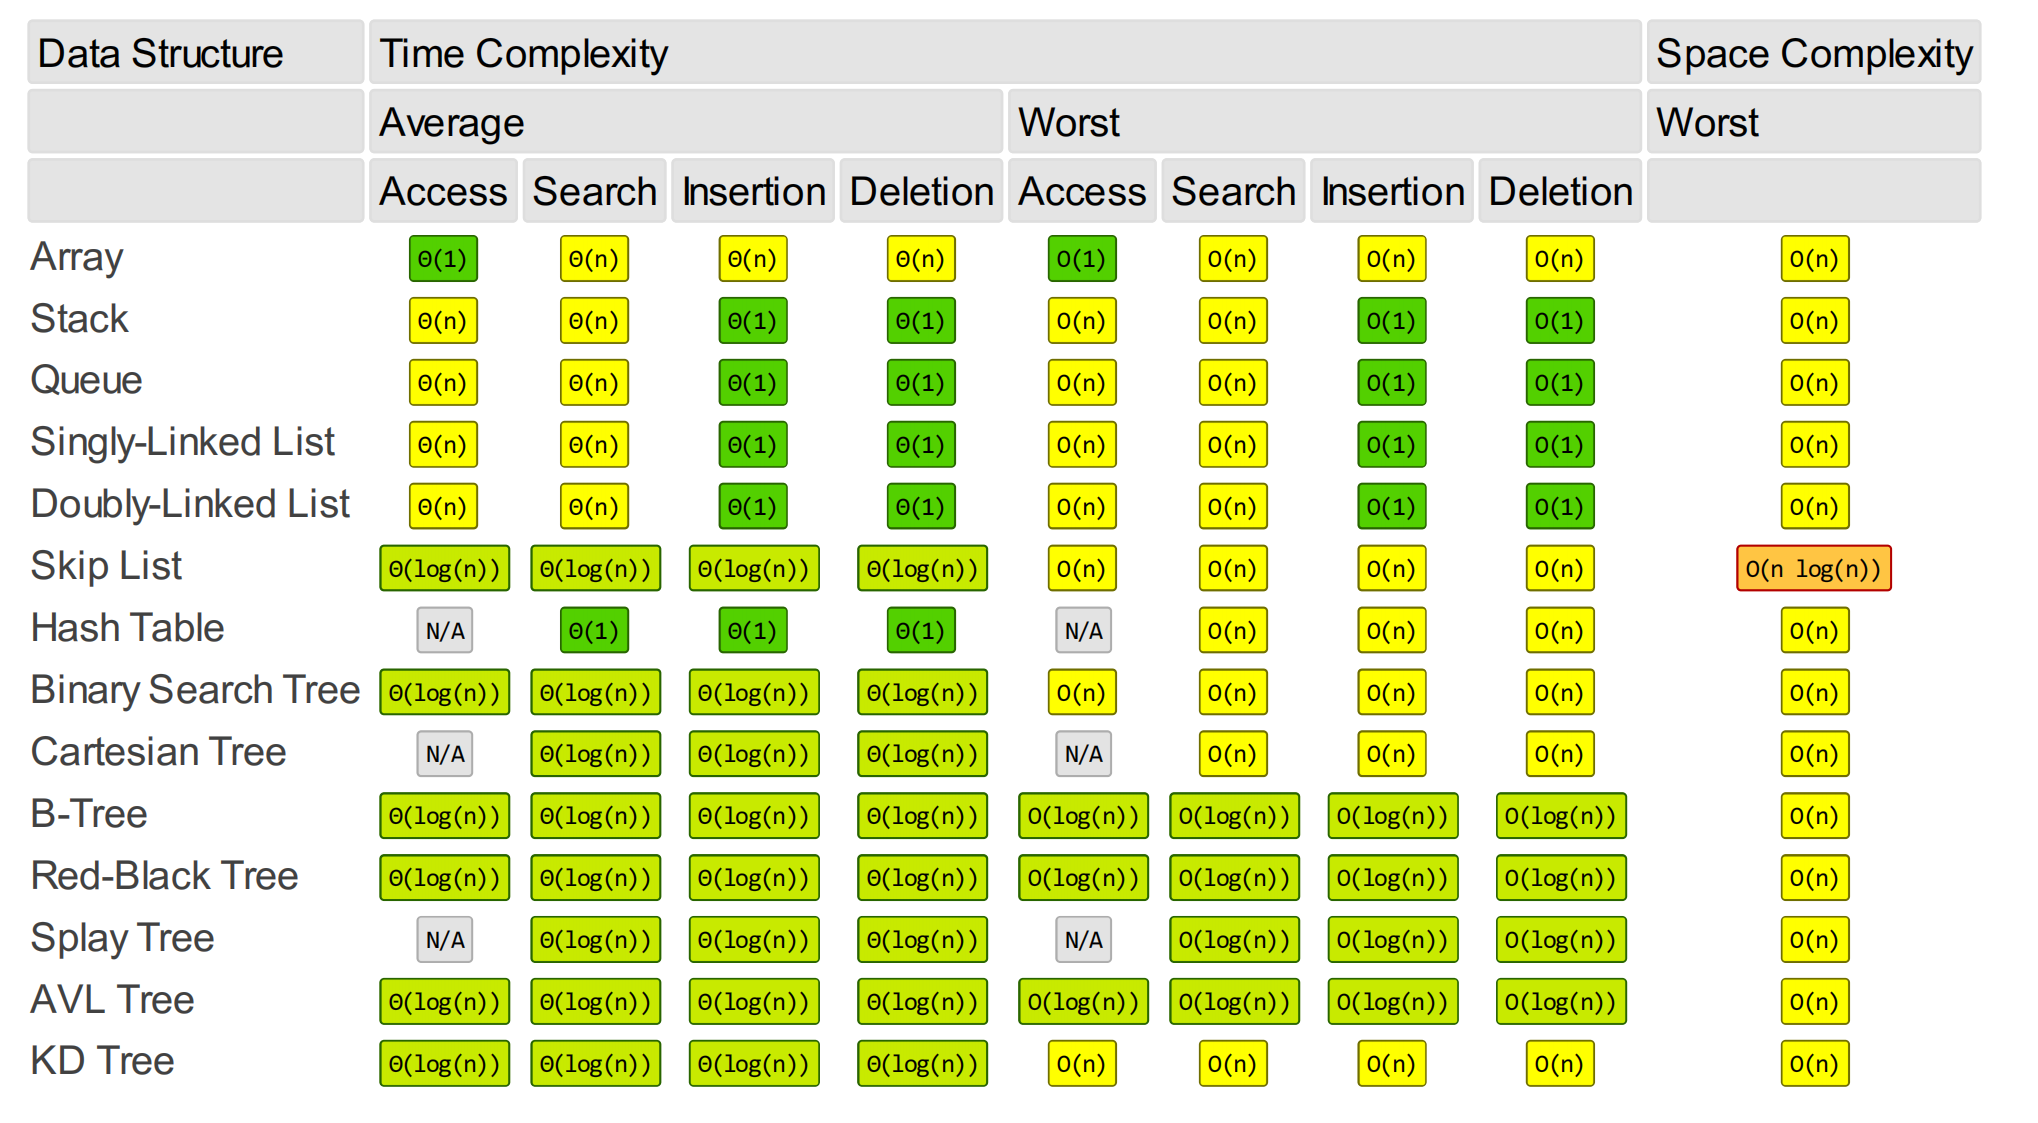
\includegraphics[width=0.9\textwidth]{images_content/1.png} %插入图片,[]中设置图片大小,{}中是图片文件名
\caption{Common Data Structure Operations} %最终文档中希望显示的图片标题
\end{figure}

\subsection{Array Sorting Algorithms}
\begin{figure}[H] %H为当前位置,!htb为忽略美学标准,htbp为浮动图形
\centering %图片居中
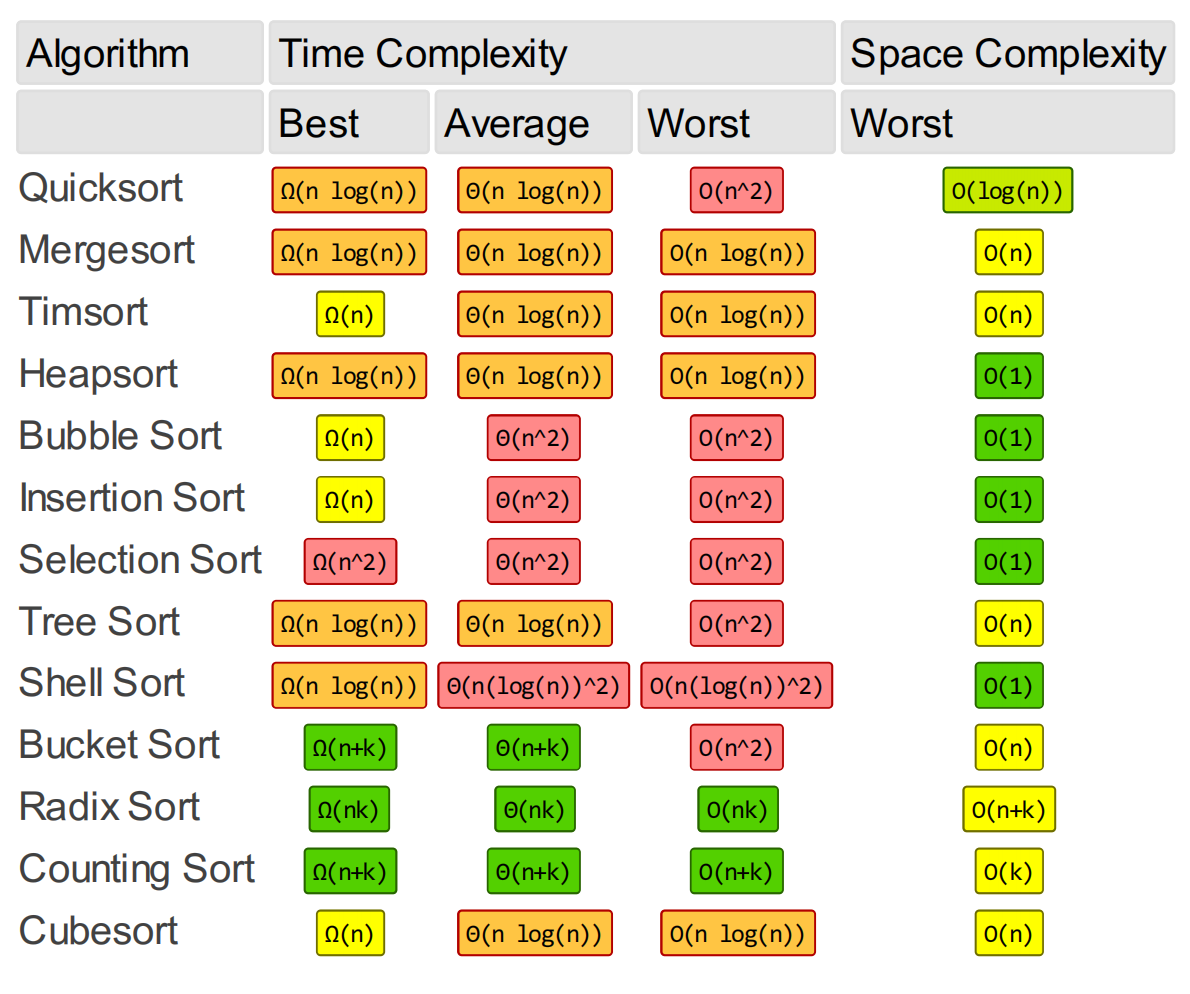
\includegraphics[width=0.7\textwidth]{images_content/2.png} %插入图片,[]中设置图片大小,{}中是图片文件名
\caption{Array Sorting Algorithms} %最终文档中希望显示的图片标题
\end{figure}

\subsection{Growth Rates}
\begin{figure}[H] %H为当前位置,!htb为忽略美学标准,htbp为浮动图形
\centering %图片居中
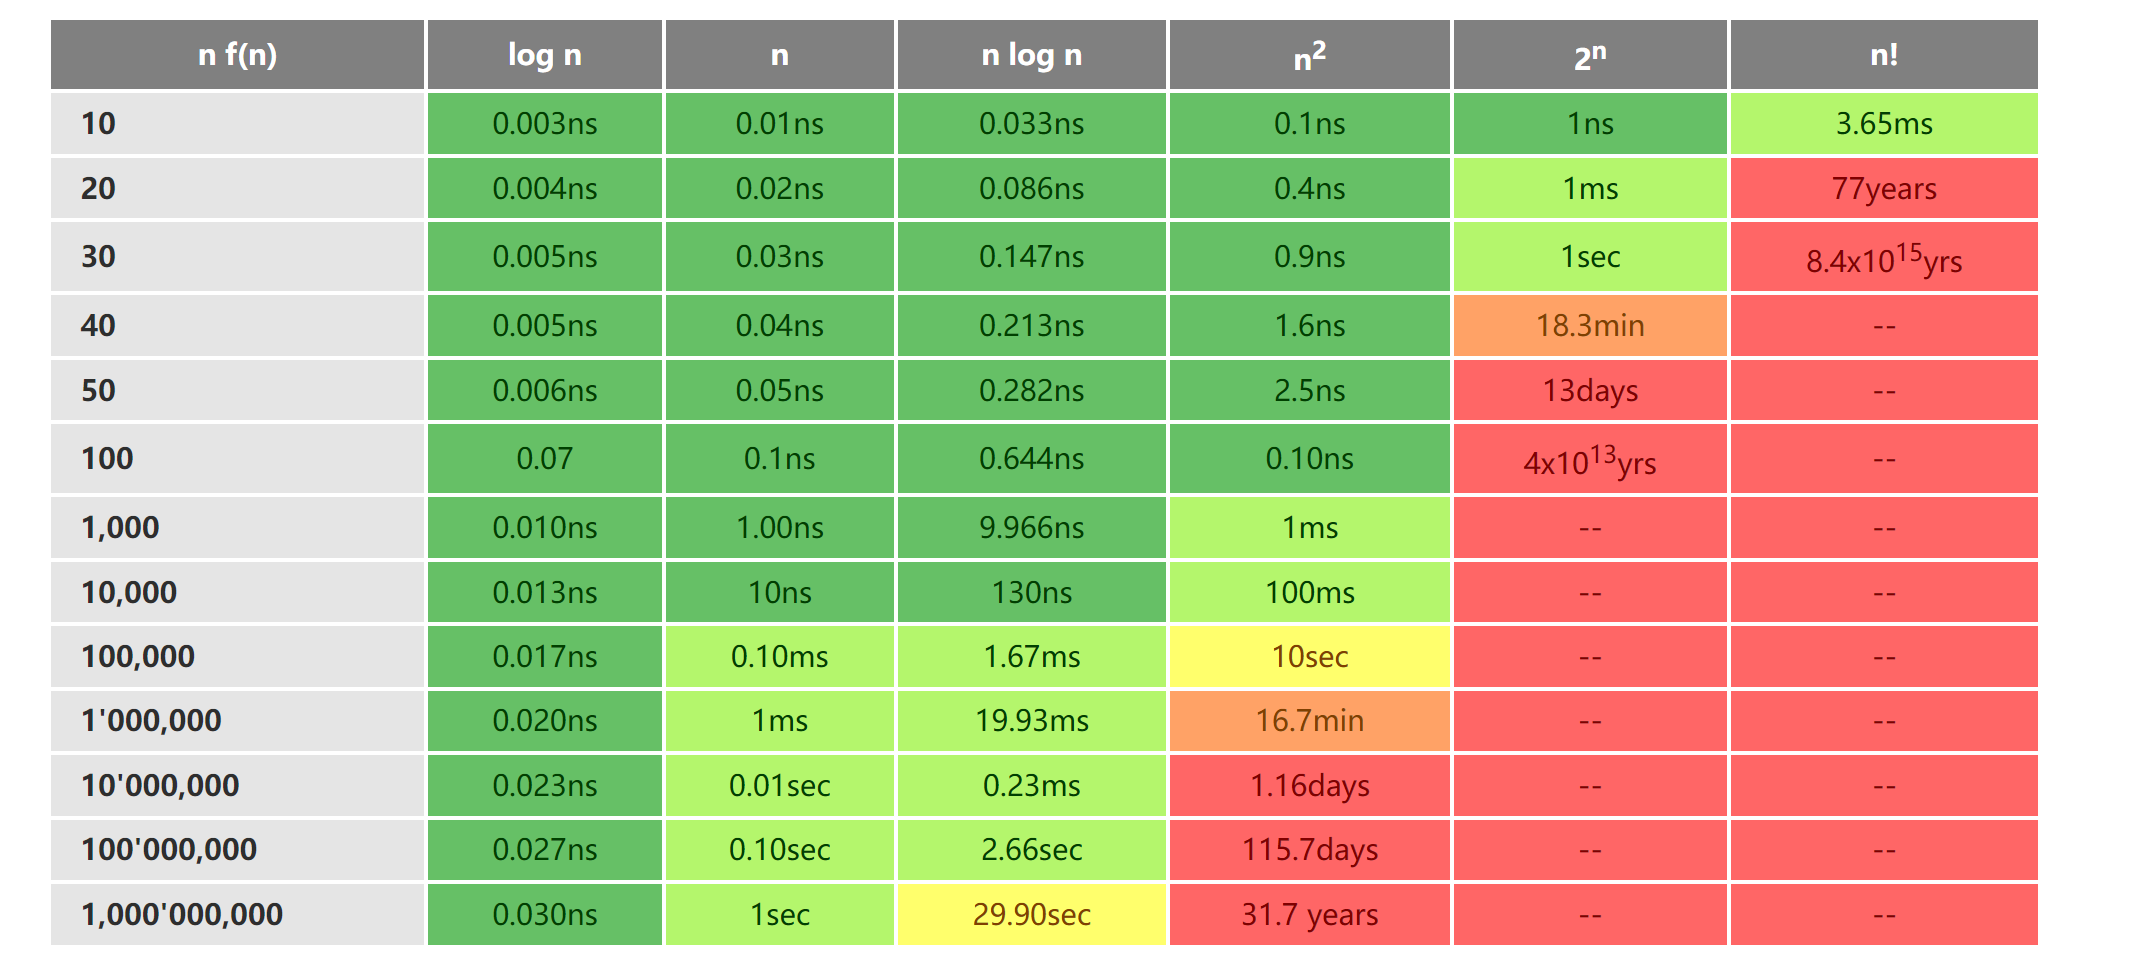
\includegraphics[width=0.9\textwidth]{images_content/3.png} %插入图片,[]中设置图片大小,{}中是图片文件名
\caption{Growth Rates} %最终文档中希望显示的图片标题
\end{figure}


\section{数据范围=>算法复杂度及算法内容}
原地址:\href{https://www.acwing.com/blog/content/32/}{https://www.acwing.com/blog/content/32/}
\begin{table}[!ht]
    \raggedleft
    \caption{由数据范围反推算法复杂度以及算法内容}
    \renewcommand\arraystretch{1.5}
    \begin{tabular}{|l|l|l|}
    \hline
        \textbf{数据范围} & \textbf{ 级别 } & \textbf{ 算法选择 } \\ \hline
        $n \le 30$ & 指数级别 & \hword{dfs+剪枝} \hword{状态压缩dp} \\ \hline
        $n \le 100$ & $O(n^3)$ & \hword{floyd} \hword{ dp } \hword{ 高斯消元 } \\ \hline
        $n \le 1000 $ & $O(n^2) O(n^2\log{n})$ & \hword{ dp } \hword{ 二分 } \hword{ 朴素版Dijkstra } \hword{ 朴素版Prim} \hword{ Bellman-Ford } \\ \hline
        $n \le 10^4$ & $O(n\sqrt{n})$  & \hword{ 块状链表 } \hword{ 分块 } \hword{ 莫队 } \\ \hline
        $n \le 10^5$ & $O(n\log{n})$ & \makecell[l]{ \hword{ 各种sort } \hword{ 线段树 } \hword{ 树状数组 } \hword{ set/map } \hword{ heap } \hword{ 拓扑排序 } \hword{ dijkstra+heap } \\ \hword{ prim+heap } \hword{ Kruskal } \hword{ spfa } \hword{ 求凸包 } \hword{ 求半平面交 } \hword{ 二分 } \hword{ CDQ分治 } \\ \hword{ 整体二分 } \hword{ 后缀数组 } \hword{ 树链剖分 } \hword{ 动态树 }} \\ \hline
        \multirow{2}*{$n \le 10^6$} & $O(n)$ & \hword{ 单调队列 } \hword{ hash } \hword{ 双指针扫描 } \hword{ 并查集 } \hword{ kmp } \hword{ AC自动机 } \\ \cline{2-3}
        & 常数较小的$O(n\log{n})$算法& \hword{ sort } \hword{ 树状数组 } \hword{ heap } \hword{ dijkstra } \hword{spfa} \\ \hline
        $n \le 10^7$  & $O(n)$ & \hword{ 双指针扫描 } \hword{ kmp } \hword{ AC自动机 } \hword{ 线性筛素数 } \\ \hline
        $n \le 10^9$ & $O(\sqrt{n})$  & \hword{ 判断质数 } \\ \hline
        $n \le 10^{18}$ & $O(\log{n})$ & \hword{ 最大公约数 } \hword{ 快速幂 } \hword{ 数位DP } \\ \hline
        $n \le 10^{1000}$ & $O((\log{n})^2)$ & \hword{ 高精度加减乘除 } \\ \hline
        $n \le 10^{100000}$ & $O(\log{k} * \log{\log{k}})$, $k$表示位数 & \hword{ 高精度加减 } \hword{ FFT/NTT } \\ \hline
    \end{tabular}
\end{table}

\end{document}